\begin{figure}[ht]
    \centering
    \begin{subfigure}{0.4\textwidth}
        \centering
        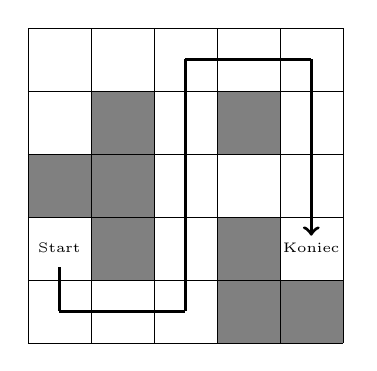
\begin{tikzpicture}[scale=0.8]
            \fill[gray] (1,2) rectangle ++(1,1);
            \fill[gray] (1,3) rectangle ++(1,1);
            \fill[gray] (3,1) rectangle ++(1,1);
            \fill[gray] (3,3) rectangle ++(1,1);
            \fill[gray] (1,1) rectangle ++(1,1);
            \fill[gray] (0,2) rectangle ++(1,1);
            \fill[gray] (3,0) rectangle ++(1,1);
            \fill[gray] (4,0) rectangle ++(1,1);

            \draw[very thick, black] (0.5,1.2) -- (0.5,0.5);
            \draw[very thick, black] (0.5,0.5) -- (2.5,0.5);
            \draw[very thick, black] (2.5,0.5) -- (2.5,4.5);
            \draw[very thick, black] (2.5,4.5) -- (4.5,4.5);
            \draw[->, very thick, black] (4.5,4.5) -- (4.5,1.7);

            \node at (0.5,1.5) {\tiny Start};
            \node at (4.5,1.5) {\tiny Koniec};

            \draw[step=1cm,ultra thin,black] (0,0) grid (5,5);
        \end{tikzpicture}
        \caption{Ścieżka nieoptymalna}
    \end{subfigure}
    \begin{subfigure}{0.4\textwidth}
        \centering
        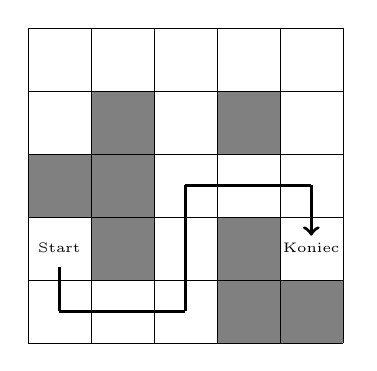
\begin{tikzpicture}[scale=0.8]
            \fill[gray] (1,2) rectangle ++(1,1);
            \fill[gray] (1,3) rectangle ++(1,1);
            \fill[gray] (3,1) rectangle ++(1,1);
            \fill[gray] (3,3) rectangle ++(1,1);
            \fill[gray] (1,1) rectangle ++(1,1);
            \fill[gray] (0,2) rectangle ++(1,1);
            \fill[gray] (3,0) rectangle ++(1,1);
            \fill[gray] (4,0) rectangle ++(1,1);

            \draw[very thick, black] (0.5,1.2) -- (0.5,0.5);
            \draw[very thick, black] (0.5,0.5) -- (2.5,0.5);
            \draw[very thick, black] (2.5,0.5) -- (2.5,2.5);
            \draw[very thick, black] (2.5,2.5) -- (4.5,2.5);
            \draw[->, very thick, black] (4.5,2.5) -- (4.5,1.7);

            \node at (0.5,1.5) {\tiny Start};
            \node at (4.5,1.5) {\tiny Koniec};

            \draw[step=1cm,ultra thin,black] (0,0) grid (5,5);
        \end{tikzpicture}
        \caption{Ścieżka optymalna}
    \end{subfigure}
    \caption{Porównanie ścieżek w labiryncie.}
    \label{fig:optimal_and_suboptimal_path}
\end{figure}